% ======================================================================
\chapter{Results and Discussion}

\section{Presentation of Results}

\subsection{Experimental setup and testing}
For the main detector we picked models on the development split and then retrained the chosen one on training and development data together, 9,513 messages in all. The numbers below come from the real test split: 1,874 messages (665 genuine, 1,209 scams) belonging to campaigns the model never saw. While designing the rules, the team also wrote 259 challenge messages. Because we wrote them ourselves, we treat them as a development check and report them separately rather than as an independent test. In the cross-domain study every setting was tuned by cross-validation on the UCI training split, every adapted model faced the same untouched Indian test set, and the whole study was run three times with seeds 42, 123 and 2026. All experiments ran on a two-core CPU with Python 3.13 and scikit-learn 1.7.2.

Testing of the software happened at three levels. First, 836 automated back-end and ML tests cover preprocessing, features, the model registry, the detector, the rules, the cross-domain service and every API route; one of them confirms that the models served by the website give exactly the notebook's scores. Another 14 tests cover the front end, and all of them pass. Second, continuous integration runs the suite on every change before it is deployed. Third, the live site is checked after each deployment.

\subsection{Main detector on ScamGuard-IN-2026}
\begin{table}[H]
\centering
\caption{Real test set, 1,874 messages from unseen campaigns (\%; FAR = false-alarm rate)}
\label{tab:final}
\begin{tabular}{|l|r|r|r|r|r|r|}
\hline
\textbf{System} & \textbf{Acc.} & \textbf{Prec.} & \textbf{Rec.} & \textbf{F1} & \textbf{FAR} & \textbf{AUC} \\
\hline
Classifier only & 97.5 & 98.6 & 97.6 & 98.1 & 2.6 & 0.997 \\
\hline
Deployed system (hand rules) & 97.1 & 98.2 & 97.2 & 97.7 & 3.2 & 0.995 \\
\hline
Learned fusion & \textbf{97.8} & \textbf{98.7} & \textbf{97.8} & \textbf{98.3} & \textbf{2.3} & 0.997 \\
\hline
\end{tabular}
\end{table}

Out of 1,209 test scams the deployed system stops 1,175, and it lets 644 of the 665 genuine messages through. Its accuracy has a 95\% confidence interval of 96.3--97.8\%, and its false-alarm rate one of 2.0--4.6\%. On the twelve messages taken from 2025--26 advisories it flags 10 of the 11 scams and leaves the one genuine notice alone, though twelve messages are far too few to conclude much.

\begin{figure}[H]
\centering
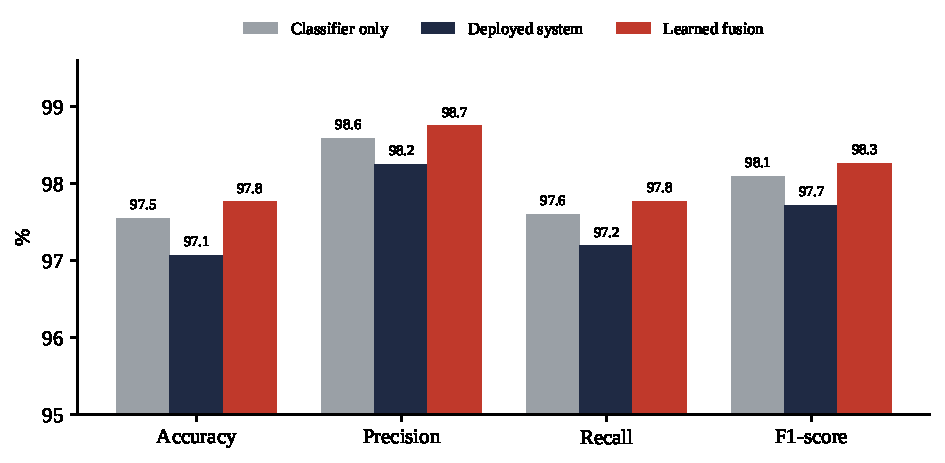
\includegraphics[width=0.62\linewidth]{figures/final_metrics.pdf}
\caption{Accuracy, precision, recall and F1-score on the real test set (vertical axis starts at 95\%)}
\label{fig:final}
\end{figure}

\textbf{Models and features.} All classifiers in Table~\ref{tab:models} share one split. Among the strong ones, logistic regression on word plus character features raises the fewest false alarms. We also tried two deep models under the same protocol. A character CNN scored 97.3\% F1 with 4.4\% false alarms and a word BiLSTM 97.4\% with 5.6\%, while logistic regression scored 97.8\% and 3.0\% in that run. Neither gap is statistically significant (McNemar $p=0.09$ and $0.11$), so the extra complexity bought nothing.

\begin{table}[H]
\centering
\caption{Classifiers on the real test set (\%); ``Challenge'' is F1 on the 259 team-written messages}
\label{tab:models}
\begin{tabular}{|l|l|r|r|r|}
\hline
\textbf{Model} & \textbf{Features} & \textbf{F1} & \textbf{False alarms} & \textbf{Challenge F1} \\
\hline
Naive Bayes & word & 96.2 & 6.2 & 88.0 \\
\hline
Naive Bayes & word + char & 95.5 & 6.5 & 86.6 \\
\hline
Logistic regression & word & 98.0 & 2.7 & 89.9 \\
\hline
Logistic regression & char & 96.9 & 4.8 & 86.8 \\
\hline
\textbf{Logistic regression} & \textbf{word + char} & \textbf{98.1} & \textbf{2.6} & 90.2 \\
\hline
Linear SVM & word & 97.7 & 5.6 & 91.6 \\
\hline
Linear SVM & word + char & 98.2 & 3.9 & 92.0 \\
\hline
Random forest & word & 97.5 & 2.7 & 73.7 \\
\hline
Random forest & word + char & 97.6 & 3.3 & 73.9 \\
\hline
\end{tabular}
\end{table}

\textbf{Label audit.} Suppose we skip the audit and call every reported message a scam. The same model then reaches 99.4\% recall, but it flags 34.0\% of genuine messages. With the audited labels, false alarms fall to 2.6\% and recall is still 97.6\%. The two models disagree on 233 test messages, and the audited one is right on 210 of them (McNemar $p<10^{-30}$, Figure~\ref{fig:audit}).

\begin{figure}[H]
\centering
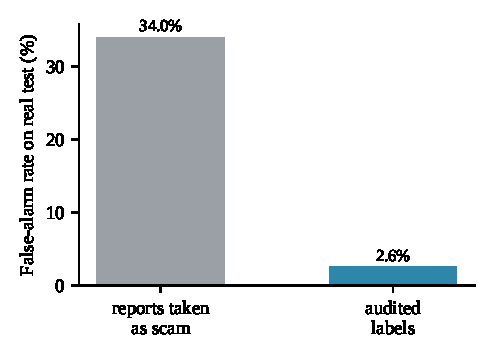
\includegraphics[width=0.5\linewidth]{figures/label_audit.pdf}
\caption{False-alarm rate with report labels and with audited labels}
\label{fig:audit}
\end{figure}

\textbf{Split and synthetic data.} When the real data is split at random, 793 test messages have a near-copy in training. That split reports 98.3\% F1 and 0.8\% false alarms; the campaign-aware split reports 97.7\% and 1.4\%. In other words, the random split hides close to half of the false alarms. Table~\ref{tab:train} changes what the model is trained on. Synthetic messages on their own are a poor stand-in for real Indian SMS. Real messages on their own catch just 35.6\% of the scams in the team-written challenge set. Using both keeps real-data F1 at 98.1\% and lifts challenge recall to 82.2\%; the price is more false alarms on real data, 2.6\% instead of 1.4\%.

\begin{table}[H]
\centering
\caption{Effect of the training data (logistic regression, word + char, \%)}
\label{tab:train}
\begin{tabular}{|l|r|r|r|r|}
\hline
\textbf{Training data} & \textbf{Real F1} & \textbf{Real FAR} & \textbf{Challenge recall} & \textbf{Challenge F1} \\
\hline
Synthetic only & 87.4 & 31.1 & 86.4 & 90.3 \\
\hline
Real only & 97.7 & 1.4 & 35.6 & 51.2 \\
\hline
Real + synthetic & 98.1 & 2.6 & 82.2 & 90.2 \\
\hline
\end{tabular}
\end{table}

\textbf{Intent rules.} The result here surprised us. On real messages from unseen campaigns, the hand-weighted rules make things slightly worse: F1 goes from 98.1\% to 97.7\% and false alarms from 2.6\% to 3.2\%. On our own challenge messages the same rules look excellent, lifting F1 from 90.2\% to 95.6\%. Weights learned from data beat the hand-set ones on real messages ($p=0.002$). We still keep the rules, but for what they actually give: phrase-level explanations and some cover for scam types missing from the real training data. They are not an accuracy gain.

\textbf{Operating point and errors.} The deployed score reaches a ROC-AUC of 0.995 (Figures~\ref{fig:rocpr} and~\ref{fig:conf}). At the default threshold it misses 34 scams and wrongly flags 21 genuine messages. Fifteen of those 21 are real bank messages that users had reported and that do ask the reader to click a link. Moving the threshold to 0.9 cuts false alarms to 1.1\% while recall drops to 92.7\%. For banking scams alone, recall is 97.7\% (895 of 916). Model and vectorizer together take 1.6~MB, training finishes in 2.7 seconds, and one message is scored in about 2~ms, or 4~ms with the rules.

\begin{figure}[H]
\centering
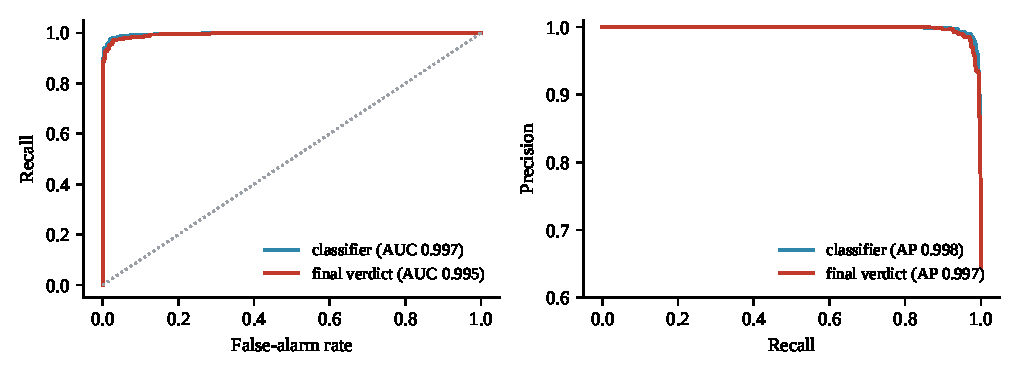
\includegraphics[width=0.95\linewidth]{figures/roc_pr.pdf}
\caption{ROC and precision--recall curves on the real test set}
\label{fig:rocpr}
\end{figure}

\begin{figure}[H]
\centering
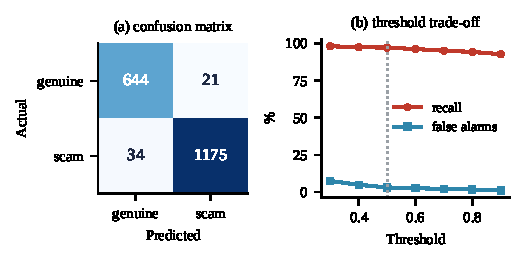
\includegraphics[width=0.7\linewidth]{figures/confusion.pdf}
\caption{(a) Confusion matrix of the deployed system; (b) recall and false-alarm rate by threshold}
\label{fig:conf}
\end{figure}

\subsection{Cross-domain generalization (RQ1 and RQ2)}
For Table~\ref{tab:cross} we took the models trained only on UCI data (seed 42) and ran them, unchanged, on all 2,050 cleaned Indian messages. Each one loses between 0.23 and 0.36 F1. The failure has a clear shape: precision is still high at 0.88--0.96, but recall sinks to 0.40--0.55. The models seldom raise a false alarm; they simply do not recognise about half of the Indian spam. Logistic Regression on word features holds up best.

\begin{table}[H]
\centering
\caption{Trained on Dataset A only (seed 42): spam F1 on the UCI test split and on all of Dataset B}
\label{tab:cross}
\begin{tabular}{|l|l|r|r|r|r|}
\hline
\textbf{Model} & \textbf{Feat.} & \textbf{F1 UCI} & \textbf{F1 India} & \textbf{Prec. India} & \textbf{Rec. India} \\
\hline
Naive Bayes & word & 0.906 & 0.551 & 0.883 & 0.401 \\
\hline
Logistic Regression & word & 0.911 & \textbf{0.678} & 0.931 & 0.533 \\
\hline
Linear SVM & word & 0.914 & 0.615 & 0.949 & 0.455 \\
\hline
Naive Bayes & char & 0.948 & 0.684 & 0.908 & 0.549 \\
\hline
Logistic Regression & char & 0.940 & 0.638 & 0.942 & 0.482 \\
\hline
Linear SVM & char & 0.943 & 0.578 & 0.956 & 0.414 \\
\hline
\end{tabular}
\end{table}

For Naive Bayes the smoothing constant decides almost everything. With the library default, $\alpha=1$, it scores 0.726 F1 on UCI and just 0.014 on Indian messages, because it calls nearly every Indian message ham. With $\alpha$ tuned on source data only, the same model scores 0.906 and 0.551.

\textbf{Why the domains differ.} About one word in five (20.7\%) of a typical Indian message never occurs in the UCI training data; for held-out UCI messages the figure is 7.8\%. Indian messages are also longer, with a median of 81 characters against 59. Links tell the same story: 87.0\% of Indian spam carries a URL, compared with 1.6\% of UCI test messages. And 24.3\% of Indian spam mentions money as ``Rs'' or ``INR'', which a UK-trained model has barely seen.

\subsection{Lightweight domain adaptation (RQ4)}
Table~\ref{tab:adapt} and Figure~\ref{fig:curve} show what labelled Indian messages do. The first 10\% of the pool does most of the work. Those 143 messages take the mean Indian F1 of Logistic Regression from 0.681 to 0.964 and that of Naive Bayes from 0.582 to 0.950, while F1 on UCI stays around 0.93. Every model, feature type and fraction improved in all three seeds, and McNemar's test gave $p<0.05$ in each of the 36 comparisons. Most of the improvement comes from spam that is now caught. For Logistic Regression at seed 42, missed spam falls from 96 messages to 3, and false alarms barely move, from 10 to 9 (Figure~\ref{fig:xcm}).

\begin{table}[H]
\centering
\caption{Spam F1 on the final Indian test set (615 messages), word TF-IDF, mean $\pm$ SD over three seeds}
\label{tab:adapt}
\begin{tabular}{|l|c|c|}
\hline
\textbf{Indian data added} & \textbf{Naive Bayes} & \textbf{Logistic Regression} \\
\hline
0\% (source-only) & 0.582 $\pm$ 0.018 & 0.681 $\pm$ 0.025 \\
\hline
10\% (143 messages) & 0.950 $\pm$ 0.006 & 0.964 $\pm$ 0.004 \\
\hline
20\% (287 messages) & 0.967 $\pm$ 0.007 & 0.968 $\pm$ 0.005 \\
\hline
40\% (574 messages) & \textbf{0.978} $\pm$ 0.009 & \textbf{0.975} $\pm$ 0.005 \\
\hline
100\% (reference only) & 0.987 $\pm$ 0.007 & 0.987 $\pm$ 0.003 \\
\hline
\end{tabular}
\end{table}

\begin{figure}[H]
\centering
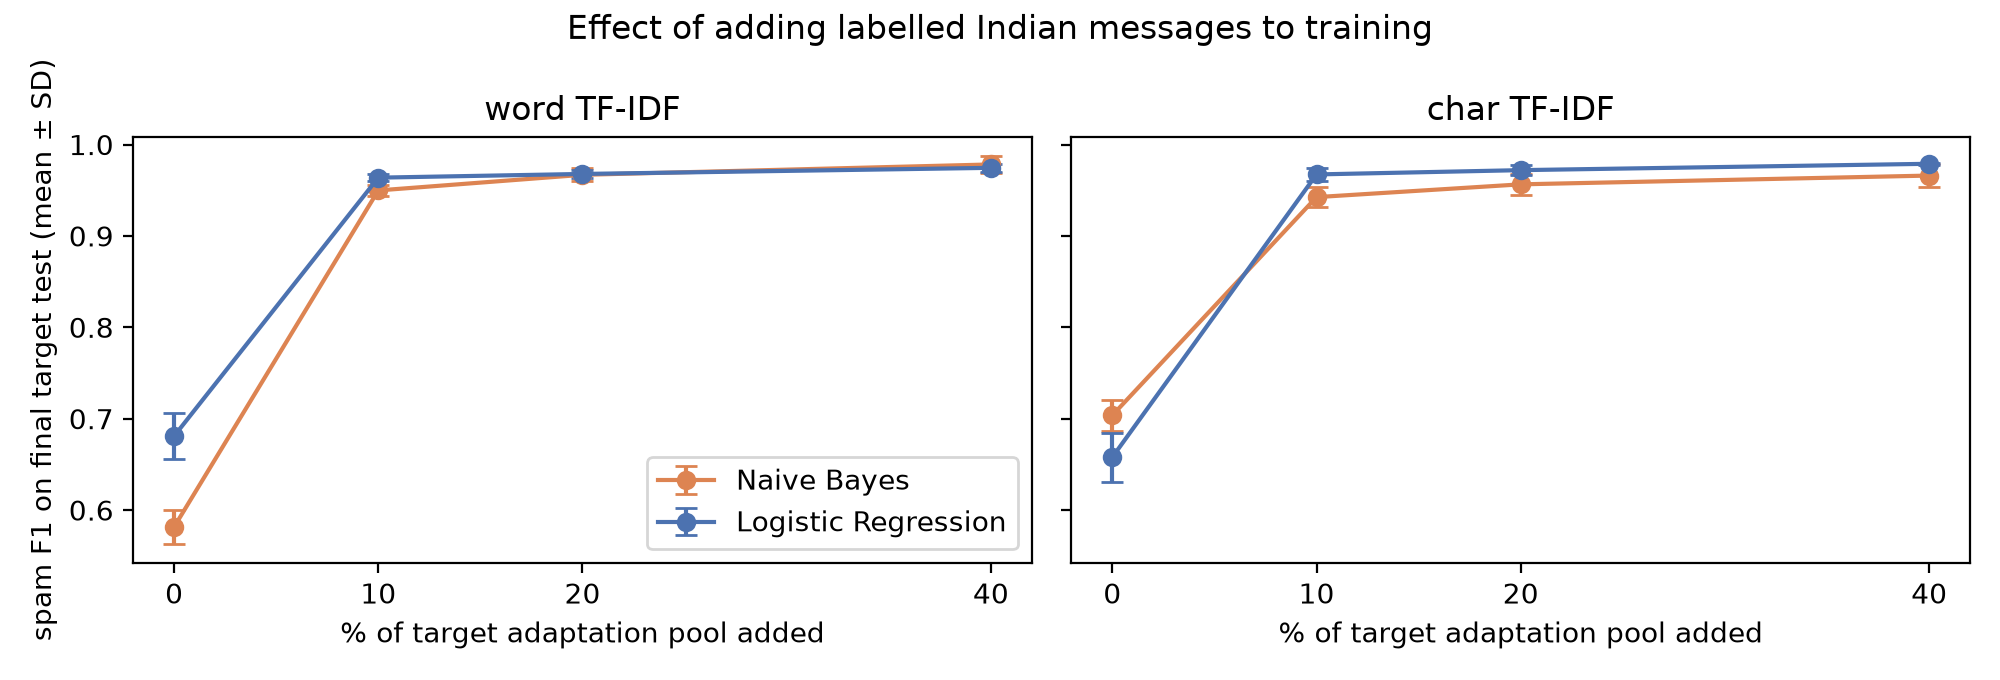
\includegraphics[width=0.95\linewidth]{figures/fig4_adaptation_curve.png}
\caption{Spam F1 on the final Indian test set as labelled Indian messages are added (mean $\pm$ SD over three seeds)}
\label{fig:curve}
\end{figure}

\begin{figure}[H]
\centering
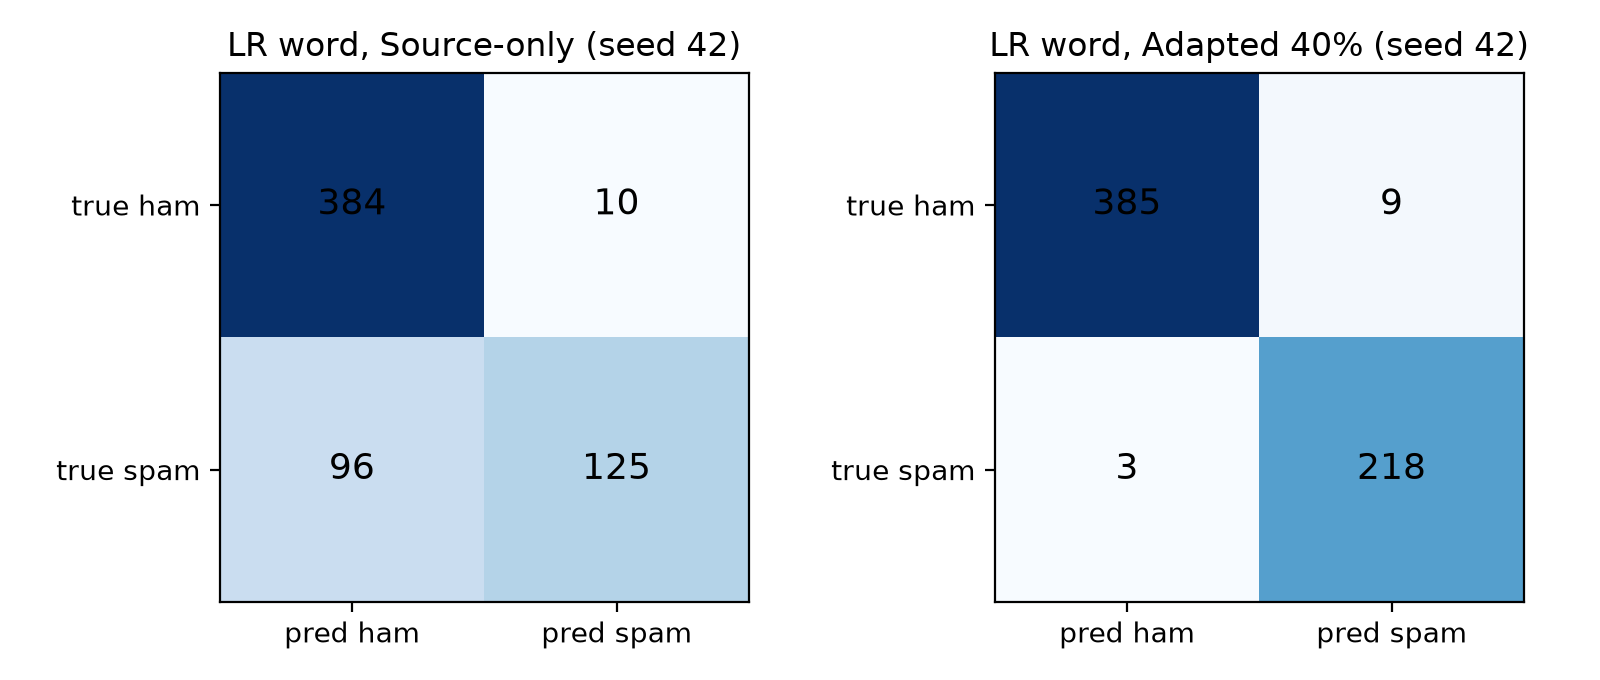
\includegraphics[width=0.8\linewidth]{figures/fig7_confusion_matrices.png}
\caption{Logistic Regression (word TF-IDF, seed 42) on the Indian test set, before and after adding 40\% of the pool}
\label{fig:xcm}
\end{figure}

\textbf{Near-duplicate check.} Indian promotions are sent from templates, so a random split may put a near-copy of a test message into the adaptation pool, and the model could then score well just by remembering it. To rule this out we grouped Dataset B with MinHash (Jaccard $\ge 0.6$) and got 1,811 groups from 2,050 messages. Under the random split, between 86 and 104 of the 615 test messages had a near-copy in the pool, depending on the seed. When we kept whole groups on one side and ran the adaptation again, the gains shrank only a little (Table~\ref{tab:group}). Memorised templates do not explain the effect.

\begin{table}[H]
\centering
\caption{Target F1 with a random and a group-aware split of Dataset B (word TF-IDF, mean $\pm$ SD)}
\label{tab:group}
\begin{tabular}{|l|l|c|c|}
\hline
\textbf{Model} & \textbf{Added} & \textbf{Random split} & \textbf{Group-aware split} \\
\hline
Logistic Regression & 0\% & 0.681 $\pm$ 0.025 & 0.652 $\pm$ 0.062 \\
\hline
Logistic Regression & 10\% & 0.964 $\pm$ 0.004 & 0.952 $\pm$ 0.008 \\
\hline
Logistic Regression & 40\% & 0.975 $\pm$ 0.005 & 0.969 $\pm$ 0.011 \\
\hline
Naive Bayes & 0\% & 0.582 $\pm$ 0.018 & 0.551 $\pm$ 0.017 \\
\hline
Naive Bayes & 10\% & 0.950 $\pm$ 0.006 & 0.937 $\pm$ 0.015 \\
\hline
Naive Bayes & 40\% & 0.978 $\pm$ 0.009 & 0.960 $\pm$ 0.015 \\
\hline
\end{tabular}
\end{table}

\subsection{Word versus character features (RQ3)}
We expected character n-grams to cope better with unfamiliar spellings, and that was only half true (Table~\ref{tab:feat}, Figure~\ref{fig:feat}). Without adaptation they lifted Indian F1 for Naive Bayes but lowered it a little for Logistic Regression. Once Indian data is added, the two feature types end up within 0.01 of each other for Logistic Regression. So neither representation wins for both classifiers.

\begin{table}[H]
\centering
\caption{Source-only models: word versus character TF-IDF (mean $\pm$ SD over three seeds)}
\label{tab:feat}
\begin{tabular}{|l|l|c|c|c|}
\hline
\textbf{Model} & \textbf{Features} & \textbf{Source F1} & \textbf{Target F1} & \textbf{Target recall} \\
\hline
Naive Bayes & word & 0.927 & 0.582 $\pm$ 0.018 & 0.430 \\
\hline
Naive Bayes & character & 0.941 & 0.704 $\pm$ 0.017 & 0.581 \\
\hline
Logistic Regression & word & 0.928 & 0.681 $\pm$ 0.025 & 0.535 \\
\hline
Logistic Regression & character & 0.942 & 0.658 $\pm$ 0.027 & 0.502 \\
\hline
\end{tabular}
\end{table}

\begin{figure}[H]
\centering
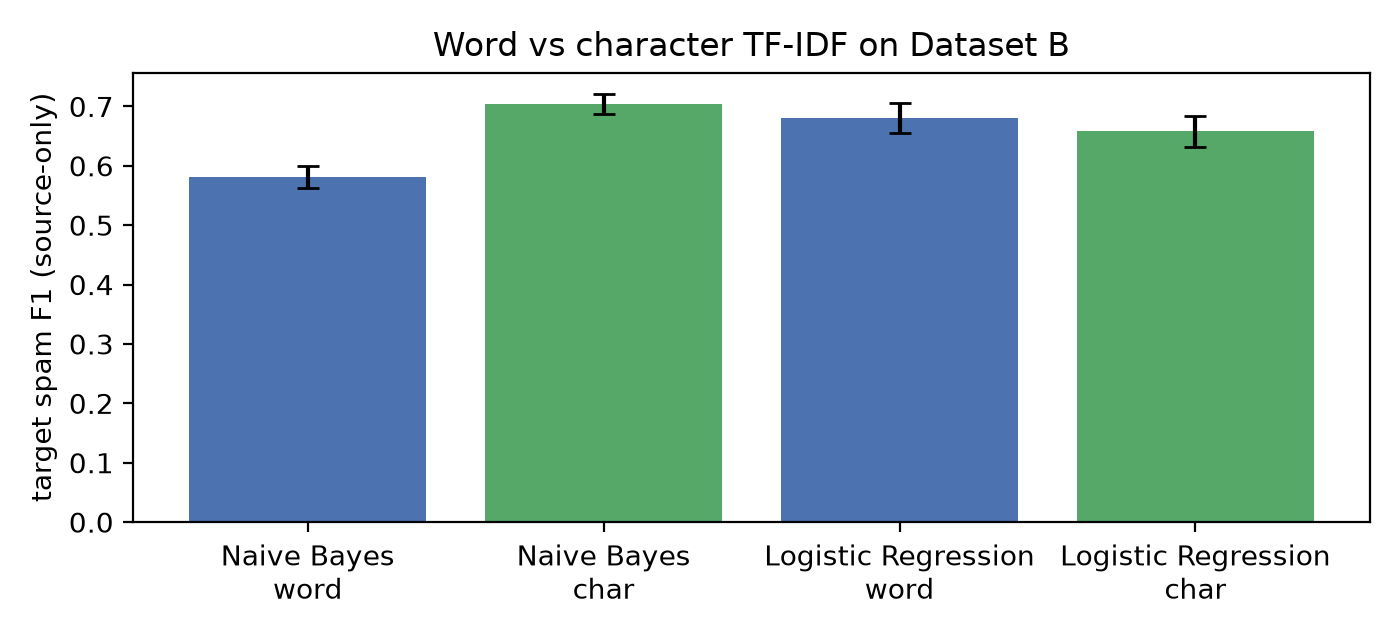
\includegraphics[width=0.7\linewidth]{figures/fig5_word_vs_char.png}
\caption{Target F1 of the source-only models with word and character TF-IDF}
\label{fig:feat}
\end{figure}

\subsection{Error analysis (RQ5)}
We read every mistake Logistic Regression (word TF-IDF, seed 42) made on the Indian test set, 106 before adaptation and 12 after, and sorted each one into a category by hand (Table~\ref{tab:errors}, Figure~\ref{fig:errors}). Before adaptation, the bulk of the errors are Indian promotions full of words the UCI model had never met. After adaptation, eight of the 12 remaining errors are tiny chat messages that give the model almost nothing to work with. We also noticed nine messages in Dataset B whose labels look doubtful to us.

\begin{table}[H]
\centering
\caption{Error categories on the Indian test set (Logistic Regression, word TF-IDF, seed 42)}
\label{tab:errors}
\begin{tabular}{|L{8.2cm}|r|r|}
\hline
\textbf{Category} & \textbf{Source-only} & \textbf{Adapted (40\%)} \\
\hline
Indian brand or telecom promotion with unfamiliar vocabulary & 61 & 0 \\
\hline
Operator service notice (data alert, pack expiry, missed call) & 14 & 0 \\
\hline
Questionable label: safety advice or receipt labelled spam & 9 & 1 \\
\hline
Very short or context-free chat (ham) & 8 & 8 \\
\hline
Fraud with disguised spelling (``t0'', ``n0w'') & 6 & 2 \\
\hline
Loan or debt message & 3 & 0 \\
\hline
Market or work commentary with spam-like words (ham) & 2 & 1 \\
\hline
Code-mixed Hinglish promotion & 2 & 0 \\
\hline
Lost characters (``????'') & 1 & 0 \\
\hline
\textbf{Total} & \textbf{106} & \textbf{12} \\
\hline
\end{tabular}
\end{table}

\begin{figure}[H]
\centering
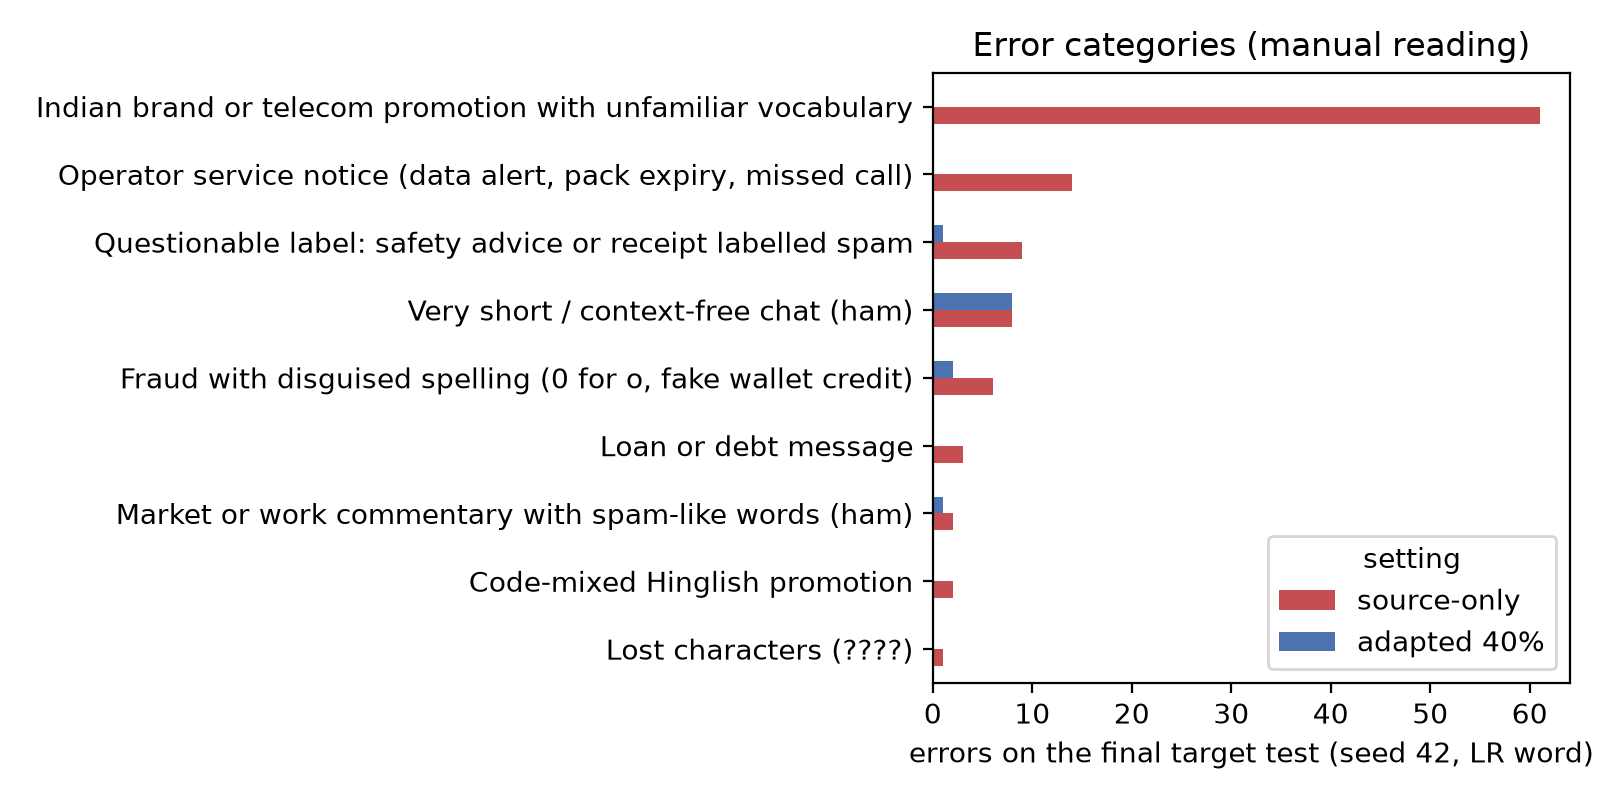
\includegraphics[width=0.8\linewidth]{figures/fig6b_error_categories_manual.png}
\caption{Error categories before and after adaptation}
\label{fig:errors}
\end{figure}

\subsection{Application}
Every functional requirement listed in Section~3.2 is available in the deployed application. On the cross-domain page a user can run one message through both the baseline and the adapted model and compare them. For example, an Indian retail offer gets 0.149 (ham) from the baseline Logistic Regression and 0.977 (spam) from the adapted one. Screenshots of the main screens are in Appendix A.

\section{Limitations of the study}
\begin{itemize}
\item \textbf{Dates of the data.} Most reported messages in ScamGuard-IN-2026 date from 2022--2024. Scam types from 2025--26 enter training only through synthetic messages and enter testing only through 12 advisory messages.
\item \textbf{How reliable the labels are.} A single annotator made the manual audit decisions, so we cannot report agreement between annotators. The Indian dataset used in the cross-domain study does not say how it was labelled, and nine of its labels look doubtful.
\item \textbf{Only two domains.} With one source and one target dataset, the study cannot claim that the findings hold for every pair of domains. Three seeds also give only a rough idea of the spread.
\item \textbf{An easy cue in Dataset B.} Not one ham message in it has a URL, whereas 87\% of its spam does. An adapted model can lean on that cue, and real messages will not always be so tidy.
\item \textbf{Disguised spellings.} The main detector's cleaner strips dotted and digit-swapped spellings before building features. The intent rules catch many such messages, but we have not tested attackers who adapt to the system.
\item \textbf{Scope.} The system judges single messages in English and Hindi only, and in the cross-domain study ``spam'' also covers legitimate promotions.
\end{itemize}

\section{Conclusion}
Three findings matter most. The labels mattered more than the model. Report labels led to 34.0\% false alarms and audited labels to 2.6\%, whereas all sensible classifiers, the CNN and BiLSTM included, landed within a few points of one another. The way we evaluate also changed the conclusions. A campaign-aware split reveals errors that a random split conceals, and rules that shine on their authors' own messages add nothing on independent data. Finally, a standard spam classifier does not travel well between countries. Trained on UK messages, it misses roughly half of Indian spam. Yet 143 labelled Indian messages bring F1 back above 0.95 without hurting UK performance, in every seed and with significance under McNemar's test.

% ======================================================================
\chapter{Conclusion}
ScamGuard spots scam and spam SMS aimed at Indian users and tells them why. Trained on our audited ScamGuard-IN-2026 corpus and tested with a campaign-aware split, the deployed detector gets 97.1\% of real messages from unseen campaigns right with 3.2\% false alarms. It replies within milliseconds and shows the exact phrases behind every verdict.

The cross-domain study that our guide proposed adds a second lesson. A classifier of the same kind, trained on another country's messages, loses about a third of its F1 on Indian SMS, and a small, carefully labelled local sample is enough to win it back. Anyone putting such a filter into service should test it on local data first and invest in a few hundred verified local labels before turning to a heavier model.

All of this runs in a live application: quick check, full analysis, Hindi support, safety tools, a cross-domain page and a Streamlit demo. Every number in this report can be regenerated from the project repository.

\textbf{Future work.}
\begin{itemize}
\item Finish collecting the team's 2026 test set and run both evaluations again on it.
\item Bring in a second annotator for the label audit and report how often the two agree.
\item Widen the cross-domain study to more target datasets and seeds, and try adaptation with less than 10\% of the pool.
\item Undo disguised spellings before features are built, and test against attackers who adapt or paraphrase.
\item Cover Kannada, Tamil, Telugu and other Indian languages, and compare small transformer models under the same protocols.
\end{itemize}
